\section{Origin}\label{ch:polar_response}
In this chapter the directional characteristics of a single loudspeaker will be thoroughly investigate. This serves as a baseline for comparison and also is essential, because the investigated loudspeaker will be used to form a speaker array in this project.\\
In general, loudspeakers tend to display different directional behaviour depending on the frequency emitted. At low frequencies they can be viewed as omnidirectional sound sources. At higher frequencies the main direction of sound emission is in line with the motion direction of the voice coil. \citep[p. 910 f.]{crocker98}
Depending on the ratio of the emitted wavelength to the diameter of the speaker, a radiation pattern with side lobes can occur. An analytic approximation to the behaviour of the speaker can be made, when analyse a vibrating piston in an infinite baffel. It is difficult to incorporate the effects of an enclosure into this model, therefore this model only takes into account the area in front of the piston.\\
There are possibilities to numerically model the sound field around a speaker in a cabinet. However in the context of this project, conducting a measurement seems to be the most favourable approach towards quantifying the sound pressure emitted by loudspeaker mounted in an enclosure for the start point for this report. Measurements must be taken at numerous frequencies and positions along a circular trajectory.
For this project, measurements are conducted by placing the test object on a turntable in free field conditions and measuring transfer functions with a microphone system. The voltage output of the amplifier and the gain of the microphone can be calibrated so that the only unknown part is the transduction performed by the \gls{dut}. The results of this measurement contain several  impulse responses in time domain and corresponding transfer functions in frequency domain. Because they  often will be visualized in polar plots, they will henceforth be referred to as the \textit{polar response}.
The knowledge gained through measuring the polar response can then be used in order to designate a feasible frequency range for beamforming. 

\section{Transfer Function Measurement with Sweeps}\label{sec:sweep_theorie}
The characterization of the directional behaviour of the speaker consists of a large number of polar response measurements. While there are many methods available to obtain polar response, it was decided to go with a method that is based on sweeps, due to several benefits. \citep[p. 3 ff.]{mueller01}\\
The sweep signal used for the measurement can be generated by the \gls{ift} of a desired spectrum and a group delay that is designed accordingly. In this project the noise spectrum is expected to be nearly pink, and therefore the sweep will be logarithmic. This results in a sinusidal waveform with a continuously altering frequency. This can ether start at low frequency and go upwards or starting in high frequency and go downwards, it can not be mixed. In most cases it is desirable to keep a nearly constant amplitude over the whole length of the sweep. The procedure of generating such a sweep signal is illustrated in \autoref{fig:sweep_signal}.

\begin{figure}[htbp]
	\centering
	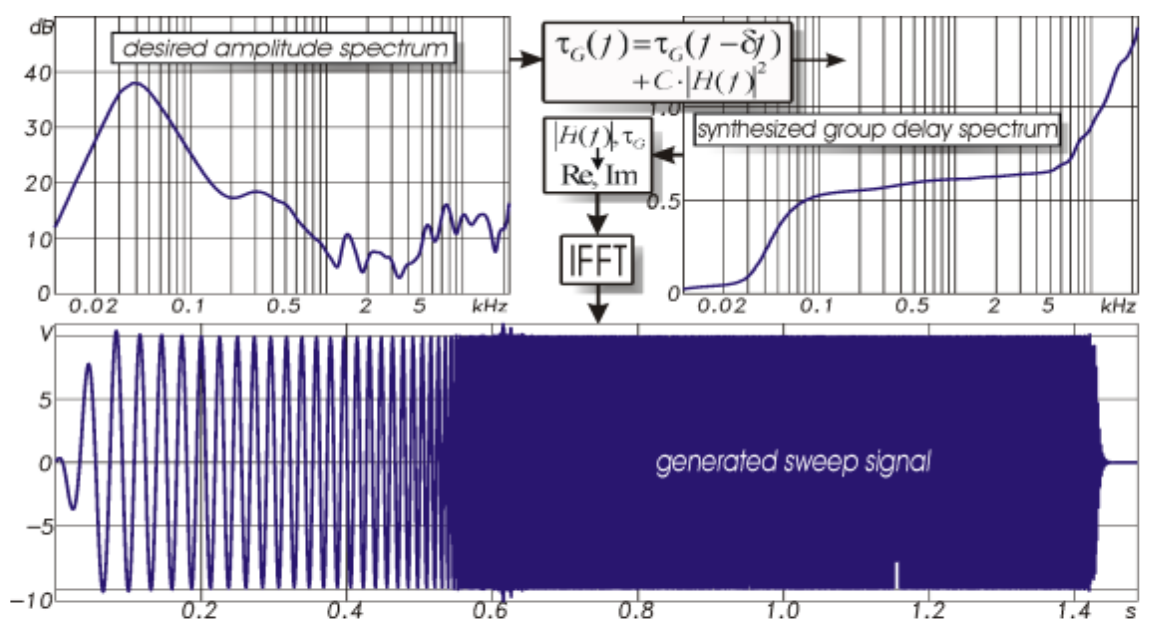
\includegraphics[width=1\textwidth]{mueller01_sweep.png}
	\caption{Sweep synthesis with arbitrary spectral magnitude and nearly constant envelope, taken from \citep{mueller01}}
		\label{fig:sweep_signal}
\end{figure}

The test signal is played back via the loudspeaker that is the \gls{dut} and the sound is recorded with a microphone in a particular angle towards the main axis of the loudspeaker. An \gls{fft} is performed on the recorded signal. The transfer function of the loudspeaker is then calculated by a multiplication operation with the recorded signal and the inverse of the test signal in frequency domain. It has to be taken into account, that not only the properties of the loudspeaker, but also the distance between the loudspeaker, the microphone and the sound field in the room have an influence on the measurement results. In the context of this project there is therefore expedient to conduct the measurements in free field conditions, which means resorting to an anechoic chamber.\\
One particular advantage of sweep measurements over other methods to determine the polar response is that nonlinearities in the measurement chain or the \gls{dut}, that lead to distortion, can be isolated from the measured transfer function and can be assessed seperately. \citep[p. 20 f.]{mueller01} Simply explained, this property is due to the fact, that in the sweep signal, every frequency has a certain group delay, which leads to harmonics being displayed at a distinct time when the test signal and the measured signal are convolved in time domain. While it is not the subject of this project to investigate nonlinearities in the behaviour of the speaker in depth, keeping track of the distortion helps with keeping the gains in the measurement chain at a good operating level.

\section{Measurement Setup}\label{sec:meas_setup}
In order to obtain the polar response, transfer functions have to be measured at numerous points. To make measurements more time efficient the loudspeaker is placed on a turntable. The acoustical center (see also \autoref{sec:ac_center}) of the loudspeaker is placed on the turning axis. The gain on the microphone amplifier and the input of the sound card are calibrated, so that a known digital value at the sound card corresponds to a known sound pressure at the microphone membrane. The gain of the power amplifier that drives the speaker is adjusted, so that a known value at the output of the sound card corresponds to a known voltage over the terminals of the speaker. With these prerequisites the transfer function can be quantified as sound pressure per voltage at a given distance. The rotation of the turntable, on which the \gls{dut} is placed, is controlled by the measurement routine on the computer. After every transfer function measurement, the orientation of the loudspeaker is altered, so that the measurement angles are evenly distributed along the circumference. The measurement data are stored, so that they can be processed into a readable form subsequently. \autoref{fig:measurement_setup} shows the measurement setup. 


\begin{figure}[H]
	\centering
\begin{picture}(0,0)%
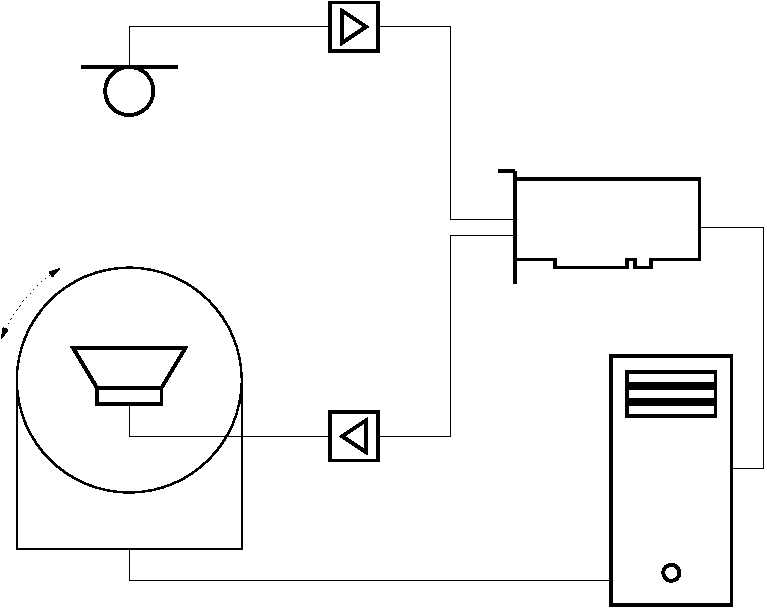
\includegraphics{meas_setup_01.pdf}%
\end{picture}%
\setlength{\unitlength}{2818sp}%
\begingroup\makeatletter\ifx\SetFigFont\undefined%
\gdef\SetFigFont#1#2#3#4#5{%
  \reset@font\fontsize{#1}{#2pt}%
  \fontfamily{#3}\fontseries{#4}\fontshape{#5}%
  \selectfont}%
\fi\endgroup%
\begin{picture}(8570,6816)(3053,-7474)
\put(4900,-1771){Microphone}%
\put(6525,-1501){Amplifier}%
\put(3250,-7081){Turntable}%
\put(6525,-6091){Amplifier}%
\put(9125,-3211){Sound Card}%
\put(10025,-6361){Computer}%
\end{picture}%
\caption{Measurement setup for transfer functions; for convenience the loudspeaker is placed on a turntable, that is controlled by the measurement routine on the computer.}
\label{fig:measurement_setup}
\end{figure}

\section{Determining the Acoustic Center of the \gls{dut}}\label{sec:ac_center}
In order to achieve meaningful results regarding the directional characteristic of the a loudspeaker, it is necessary to know the location of the  acoustic center of the loudspeaker.
In \citep{ansis1.1}, the ``effective acoustical center'' of an electroacoustical transducer is defined as the ``position of the effective or virtual point source from which sound pressure varies inversely as distance''. This concept is further discussed in \citep{jacobsenetal}, where the authors also state, that the position of the acoustic center is frequency dependent. For gathering the data to characterize the directivity it is desirable to position the acoustic center of the \gls{dut} on the rotational axis on the turntable. This can lead to practical difficulties due to the frequency dependency. It is therefore necessary to assess the position of the acoustical center of the \gls{dut} in the desired frequency range via a measurement.\\
Appendix \ref{ax:directional_1} shows the results of a measurement of the polar response that has been conducted without knowing the position of the acoustic center of the \gls{dut}, the test object was a \citep{seas33}. 
\begin{figure}[htbp]
	\centering
	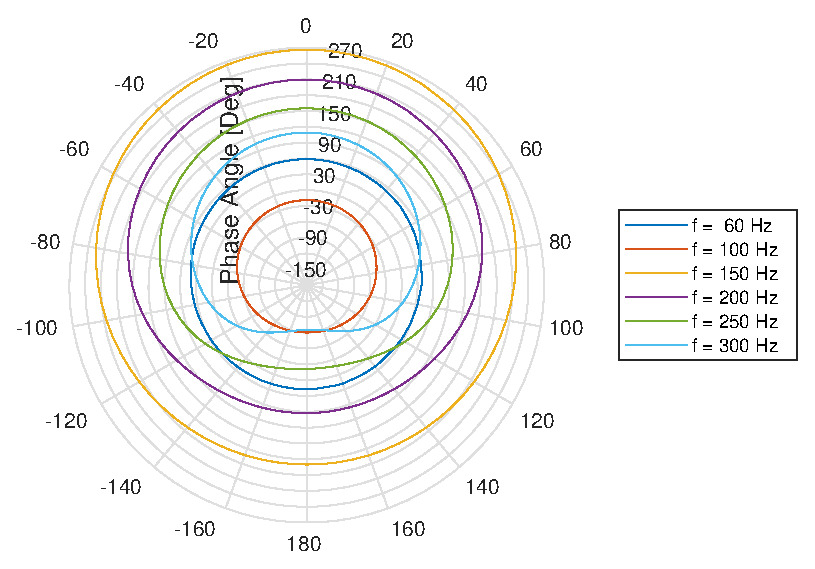
\includegraphics[width=0.7\textwidth]{02_23_phase.eps}
	\caption{Phase (uncalibrated), measured at a distance \(d=\)\SI{0.75}{\meter}, see Appendix \ref{ax:directional_1}}
		\label{fig:02_23_phase_main_part}
\end{figure}
When analyzing the phase data plotted in \autoref{fig:02_23_phase_main_part} it seems rather obvious, that the acoustic center of the \gls{dut} has been in front of the rotational axis of the turntable. 
It appears to be possible to estimate the position of the acoustic center by exploiting, that both wavelength and phase at the measurement points on the main axis (\SI{0}{\degree}) and in the opposite direction are known. As described beforehand, the concept of an acoustical center is tied to a  point source, from which waves appear to emerge. If the acoustical center is placed  on the rotational axis, the phase at all microphone positions should have the same value. In the given case it is assumed, that the acoustical center is only off the rotational axis in only the direction of the main axis of the \gls{dut}, and not shifted to the side.
The difference of the phase angles at \SI{0}{\degree} and \SI{180}{\degree} at a given frequency therefore corresponds to a proportion of the wavelength that is double of the distance that the \gls{dut} has to be shifted backwards in order to move the acoustical center onto the rotational axis.
\begin{equation}
S\,=\,\frac{1}{2}\cdot\frac{\phi_0-\phi_{180}}{360^\circ}\cdot\lambda
\end{equation}
\startexplain
    \explain{$S$ is the distance that the \gls{dut} has to be shifted backwards}{\si{m}}
    \explain{$\phi_0$ is the phase angle at the main axis}{\si{\degree}}
    \explain{$\phi_{180}$ is the phase angle at \SI{180}{\degree}}{\si{\degree}}
    \explain{$\lambda$ wavelength}{\si{m}}
\stopexplain    
If \(S\) takes on a negative value, the acoustical center is behind the rotational axis and the \gls{dut} has to be shifted towards the front. There are constraints to the applicability of this concept. The frequency, on which the calculation is based, has to be inside the frequency range at which the speaker can be considered omnidirectional.
The wavelength of the measured frequency can be problematic when it is very long, as the phase difference \(\delta\phi\) between \(\phi_0\) and \(\phi_{180}\) becomes comparatively small. This leads to a bigger influence to the uncertainty of the phase measurement. On the other hand, comparatively short wavelengths may lead to aliasing effects, when there is a big offset of the center from the rotational axis. However this is not relevant in this practical application, because towards higher frequencies, loudspeakers tend not to behave like omnidirectional sources.\\
In \autoref{tab:shift_meas1}, data from the measurement described in Appendix \ref{ax:directional_1} has been used to calculate the offset of the acoustical center from the rotational axis of the turntable at three different frequencies. The wavelengths \(\lambda\) were based on the assumption, that the speed of sound was \(c\,=\,\)\SI{343}{\meter\per\second}, corresponding to a temperature \(T\,\approx\,\)\SI{20}{\celsius}. The results for all three frequencies are rather similar.
\begin{table}[H]
\centering
\caption{Calculation of the offset of the acoustic center based on Appendix \ref{ax:directional_1}}
\label{tab:shift_meas1}
\begin{tabular}{|lr|r|r|r|}
\hline
Frequency              & {[}Hz{]}  & 60    & 100    & 150    \\ \hline
\(\phi_0\)             & {[}Deg{]} & 58.8  & 341.1  & 266.1  \\ \hline
\(\phi_{180}\)         & {[}Deg{]} & 17.2  & 269.7  & 159.9  \\ \hline
\(\Delta\phi\)         & {[}Deg{]} & 41.6  & 71.4   & 106.2  \\ \hline
\(\lambda\)            & {[}m{]}   & 5.72  & 3.43   & 2.29   \\ \hline
\(S\)                  & {[}m{]}   & 0.330 & 0.340  & 0.337  \\ \hline
\end{tabular}
\end{table}
Comparing \(S\) with the positioning of the speaker relative to the rotational axis during the measurement would allow for specifying the estimated position of the acoustic center. However, there was some significant undesired mechanical flexibility in the way the speaker was mounted, which lead to imprecisions (see \autoref{fig:setup_02_23}). Therefore, another mechanical solution was implemented and the measurement was repeated. This is  logged in Appendix \ref{ax:directional_2}.
During this second measurement campaign the speaker was placed further to the back to get the acoustical center closer to the rotational axis. However, there is still some offset, as can be seen in \autoref{tab:shift_meas2}.
Adding \(S\) to the distance between the front plane of the cabinet and the rotational axis, a rough estimate of the position of the acoustic center in relation to the front plane of the cabinet \(C\,\approx\,\)\SI{0.17}{\meter} can be made. As there were still some mechanical weaknesses involved and the temperature during the measurement was unknown, this estimate has to be confirmed in a final measurement campaign, where the speaker is set back according to the findings of \autoref{tab:shift_meas2}.\\
\begin{table}[H]
\centering
\caption{Calculation of the offset of the acoustic center based on Appendix \ref{ax:directional_2}}
\label{tab:shift_meas2}
\begin{tabular}{|lr|r|r|r|}
\hline
Frequency              & {[}Hz{]}  & 60    & 100    & 150   \\ \hline
\(\phi_0\)             & {[}Deg{]} & 108.9 & - 60.8 & 138.0 \\ \hline
\(\phi_{180}\)         & {[}Deg{]} & 103.3 & - 70.8 & 126.5 \\ \hline
\(\Delta\phi\)         & {[}Deg{]} & 5.6   & 10     & 11.5  \\ \hline
\(\lambda\)            & {[}m{]}   & 5.72  & 3.43   & 2.29  \\ \hline
\(S\)                  & {[}m{]}   & 0.044 & 0.048  & 0.037 \\ \hline
\end{tabular}
\end{table}

One aspect that has to be considered in this context is the dependency of the acoustic center on frequency. As stated in \autoref{ch:intro} the frequency range that this project deals with is \SIrange{60}{300}{\hertz}. Considering the findings of \citep{vanderkooy10}, who has done a boundary-element calculation of the acoustic center, it is assumed, that the frequency dependent position change can be deemed  negligible in the context of the formerly mentioned frequency range. 
\autoref{fig:vanderkooy_center} shows the simulated acoustic center from \citep{vanderkooy10}. The driver dimensions and cabinet layout deviate from the \gls{dut}. However, a qualitative tendency can be derived. The position of the acoustic centre appears to be relatively stable at lower frequencies. As the frequency increases, the distance between the center and the driver and the center starts increasing. At a given frequency, that happens to be around \SI{500}{\hertz} in the Vanderkooy-simulation, the distance starts decreasing significantly. This however is also described in the article, as a frequency range, in which the concept of an acoustical center is not valid anymore, due to the speaker not behaving like an omnidirectional source. The method of determining the acoustic center based on a the polar respone, as it has been described previously, should therefore deliver a sufficient approximation of the position of the acoustic center at in the frequency range, in which the concept can be viably applied.
\begin{figure}[htbp]
	\centering
	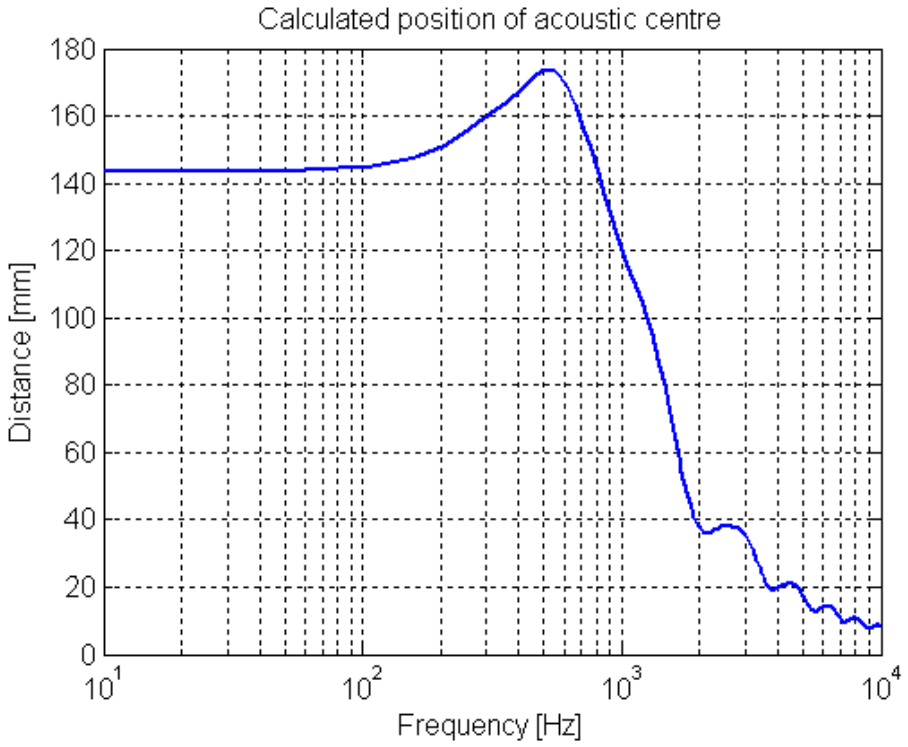
\includegraphics[width=0.7\textwidth]{vanderkooy_center.png}
	\caption{Simulated position of the acoustic center over frequency, taken from \citep{vanderkooy10}. The simulation was carried out for a piston source with radius \(r_{piston}\,=\,\)\SI{100}{\milli\meter} mounted in the flat end of a cylinder with radius $r_{cylinder}\,=\,$\SI{200}{\milli\meter} and a length $l_{cylinder}\,=\,$\SI{300}{\milli\meter}}

		\label{fig:vanderkooy_center}
\end{figure}

%A way to determine the acoustical center by measurement can be proposed as follows. The loudspeaker is placed on the turntable, oriented with its main axis directly towards the measurement microphone (\SI{0}{\degree}). Details about this procedure can be found in \autoref{ax:directional_1}.

\section{Sensitivity of the \gls{dut}}
The aim of this section is to show the usable frequency range of the specified \gls{dut}, which will be used in this project. The sensitivity can be defined as the pressure at a specified distance to the \gls{dut} while knowing the applied voltage over the \gls{dut}. The \gls{dut} is placed such that its main axis is pointing towards the microphone. The sensitivity graph can be used to illustrate the range where equalising is necessary in order to achieve a linear response and the usable frequency range of the \gls{dut}. The range where in which the pressure does not diverge significantly is the usable range, where the frequencies, at which pressure starts dropping significantly, are the limits of this range. Outside the limits, the \gls{dut} requires heavy equalising or is not able to produce the signal with a meaningful amplitude at all. The \gls{dut} might be less efficiency outside the limits and by applying heavy equalising the heat dispersion will raise and may damage the \gls{dut}. \autoref{fig:speaker_sensitivityl} shows the sensitivity for the \citep{seas33} at a distance of \SI{2.74}{\meter} with an applied \gls{rms} voltage of \SI{10.5}{\volt}


\begin{figure}[H]
	\centering
	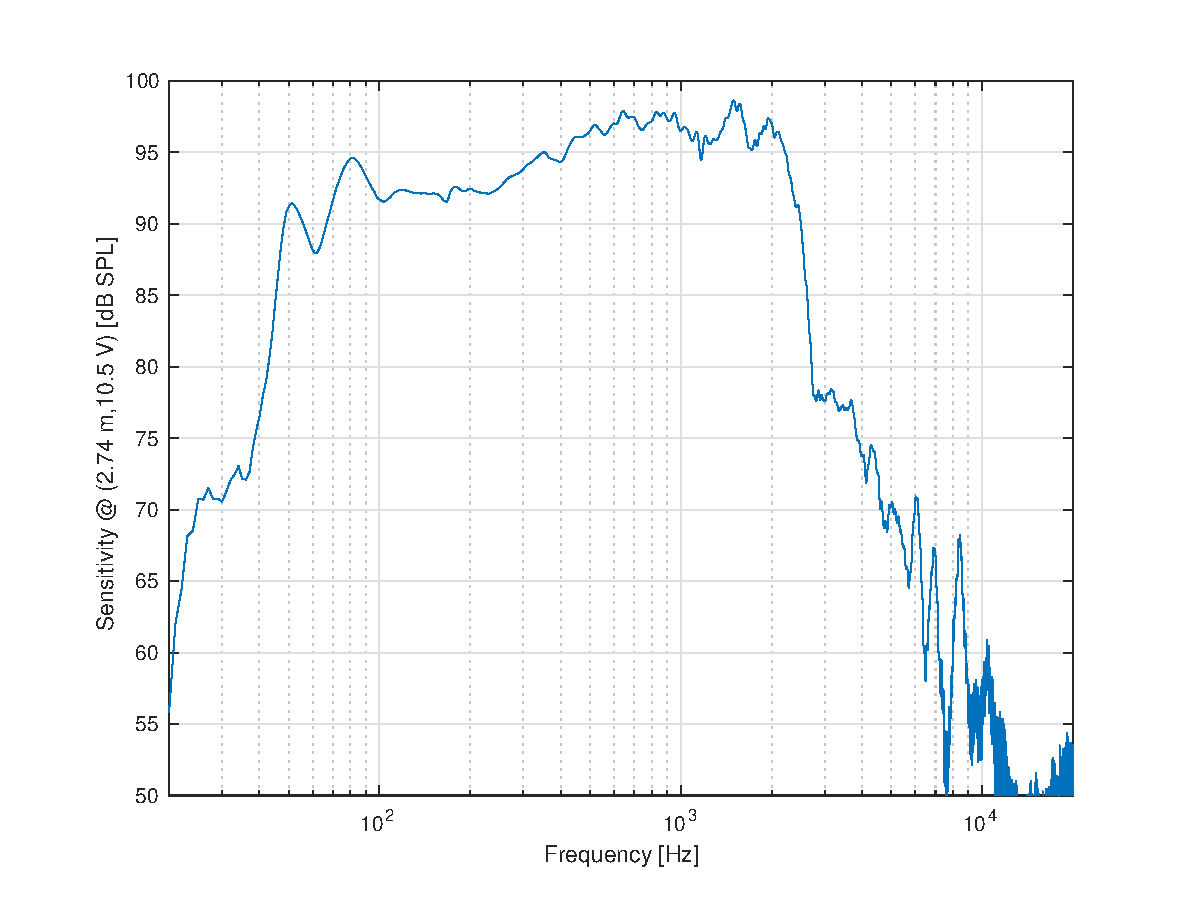
\includegraphics[width=1\textwidth]{sensitivity_seas}
	\caption{The figure shows the sensitivity @ (\SI{2.74}{\meter},\SI{10.5}{\volt}) of  \citep{seas33}}
		\label{fig:speaker_sensitivityl}
\end{figure}

The usable area of the \citep{seas33} is at least within \SI{48}{\hertz} to \SI{2.5}{\kilo\hertz} while visually analyzes \autoref{fig:speaker_sensitivityl}.


\section{Determining the beamwidth of the \gls{dut}}\label{sec:beamwidth}
The beamwidth can be defined as the range between the angles, at which the sound pressure radiated at a given frequency equals a certain threshold related to the pressure on the main axis of a speaker. In other words, because the speaker tends to be omnidirectional in low frequency and non omnidirectional in high frequency, beamwidth boundaries line describe the frequency where the pressure is decreased to the threshold. The beamwidth is strongly dependent on frequency and can be determined of the measurement data from the polar response. \autoref{fig:beamwidth_offset_4.5_cm} visualizes the beamwidth by processed the measurement data from \ref{ax:directional_2} with the descried calculation in \autoref{appendix:beamwidth}. It has to be noted, that during this measurement the acoustic center of the \gls{dut} was not placed exactly on the rotational axis of the speaker. The beamwith is therefore slightly smaller then it would have been, if the center were matching.

\begin{figure}[H]
	\centering
	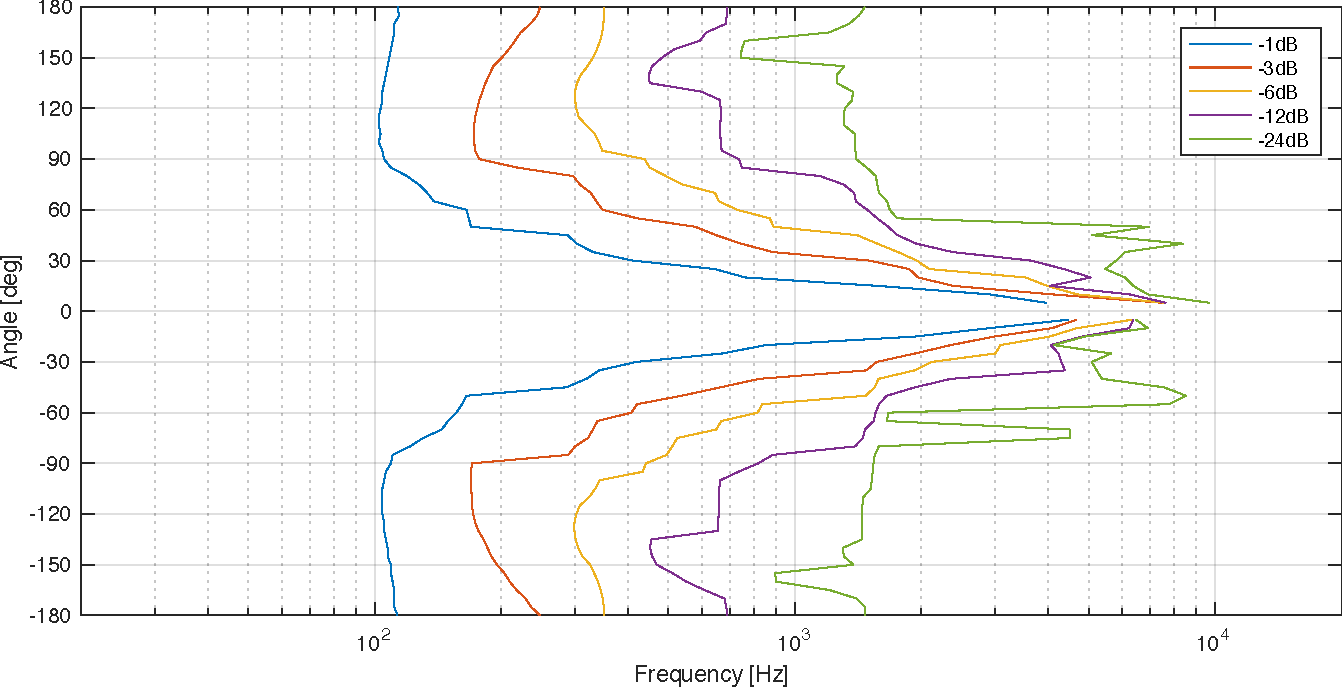
\includegraphics[width=1\textwidth]{beamwidth_off_4_5_cm.pdf}
	\caption{The figure shows the beamwidth to a specified \si{\decibel} change between the front measurement and a measurement from a given angle of the \gls{dut}. It find the first frequency where the \gls{spl} difference between front measurement and the measurement from the given angle is $n$\,\si{\decibel}, where $n$ is given in the legend. The \gls{dut} which correspond to this figure is a \citep{seas33}}
		\label{fig:beamwidth_offset_4.5_cm}
\end{figure}